\subsection{Interpretador \textit{Tree-Walking}}

Um interpretador é um programa que executa diretamente o código fonte de uma linguagem de programação, linha por linha. No caso deste trabalho, será utilizada a variante \textit{tree-walking}, que simplifica o método de execução do interpretador ao custo de desempenho \cite{craftinginterpreters}. Esta variante se adequa ao objetivo do trabalho, que visa a implementação de um protótipo simples, sem preocupações com desempenho.

Interpretadores \textit{tree-walking} podem ser divididos em quatro fases sequenciais: análise léxica, análise sintática, análise semântica, e por fim, interpretação \cite{craftinginterpreters}. Cada fase, com exceção da interpretação, gera um produto que é posteriormente processado pela fase seguinte.

A \autoref{fig:mapa_interpretador} ilustra alguns dos principais caminhos que um interpretador pode seguir.

\begin{figure}[H]
	\centering
	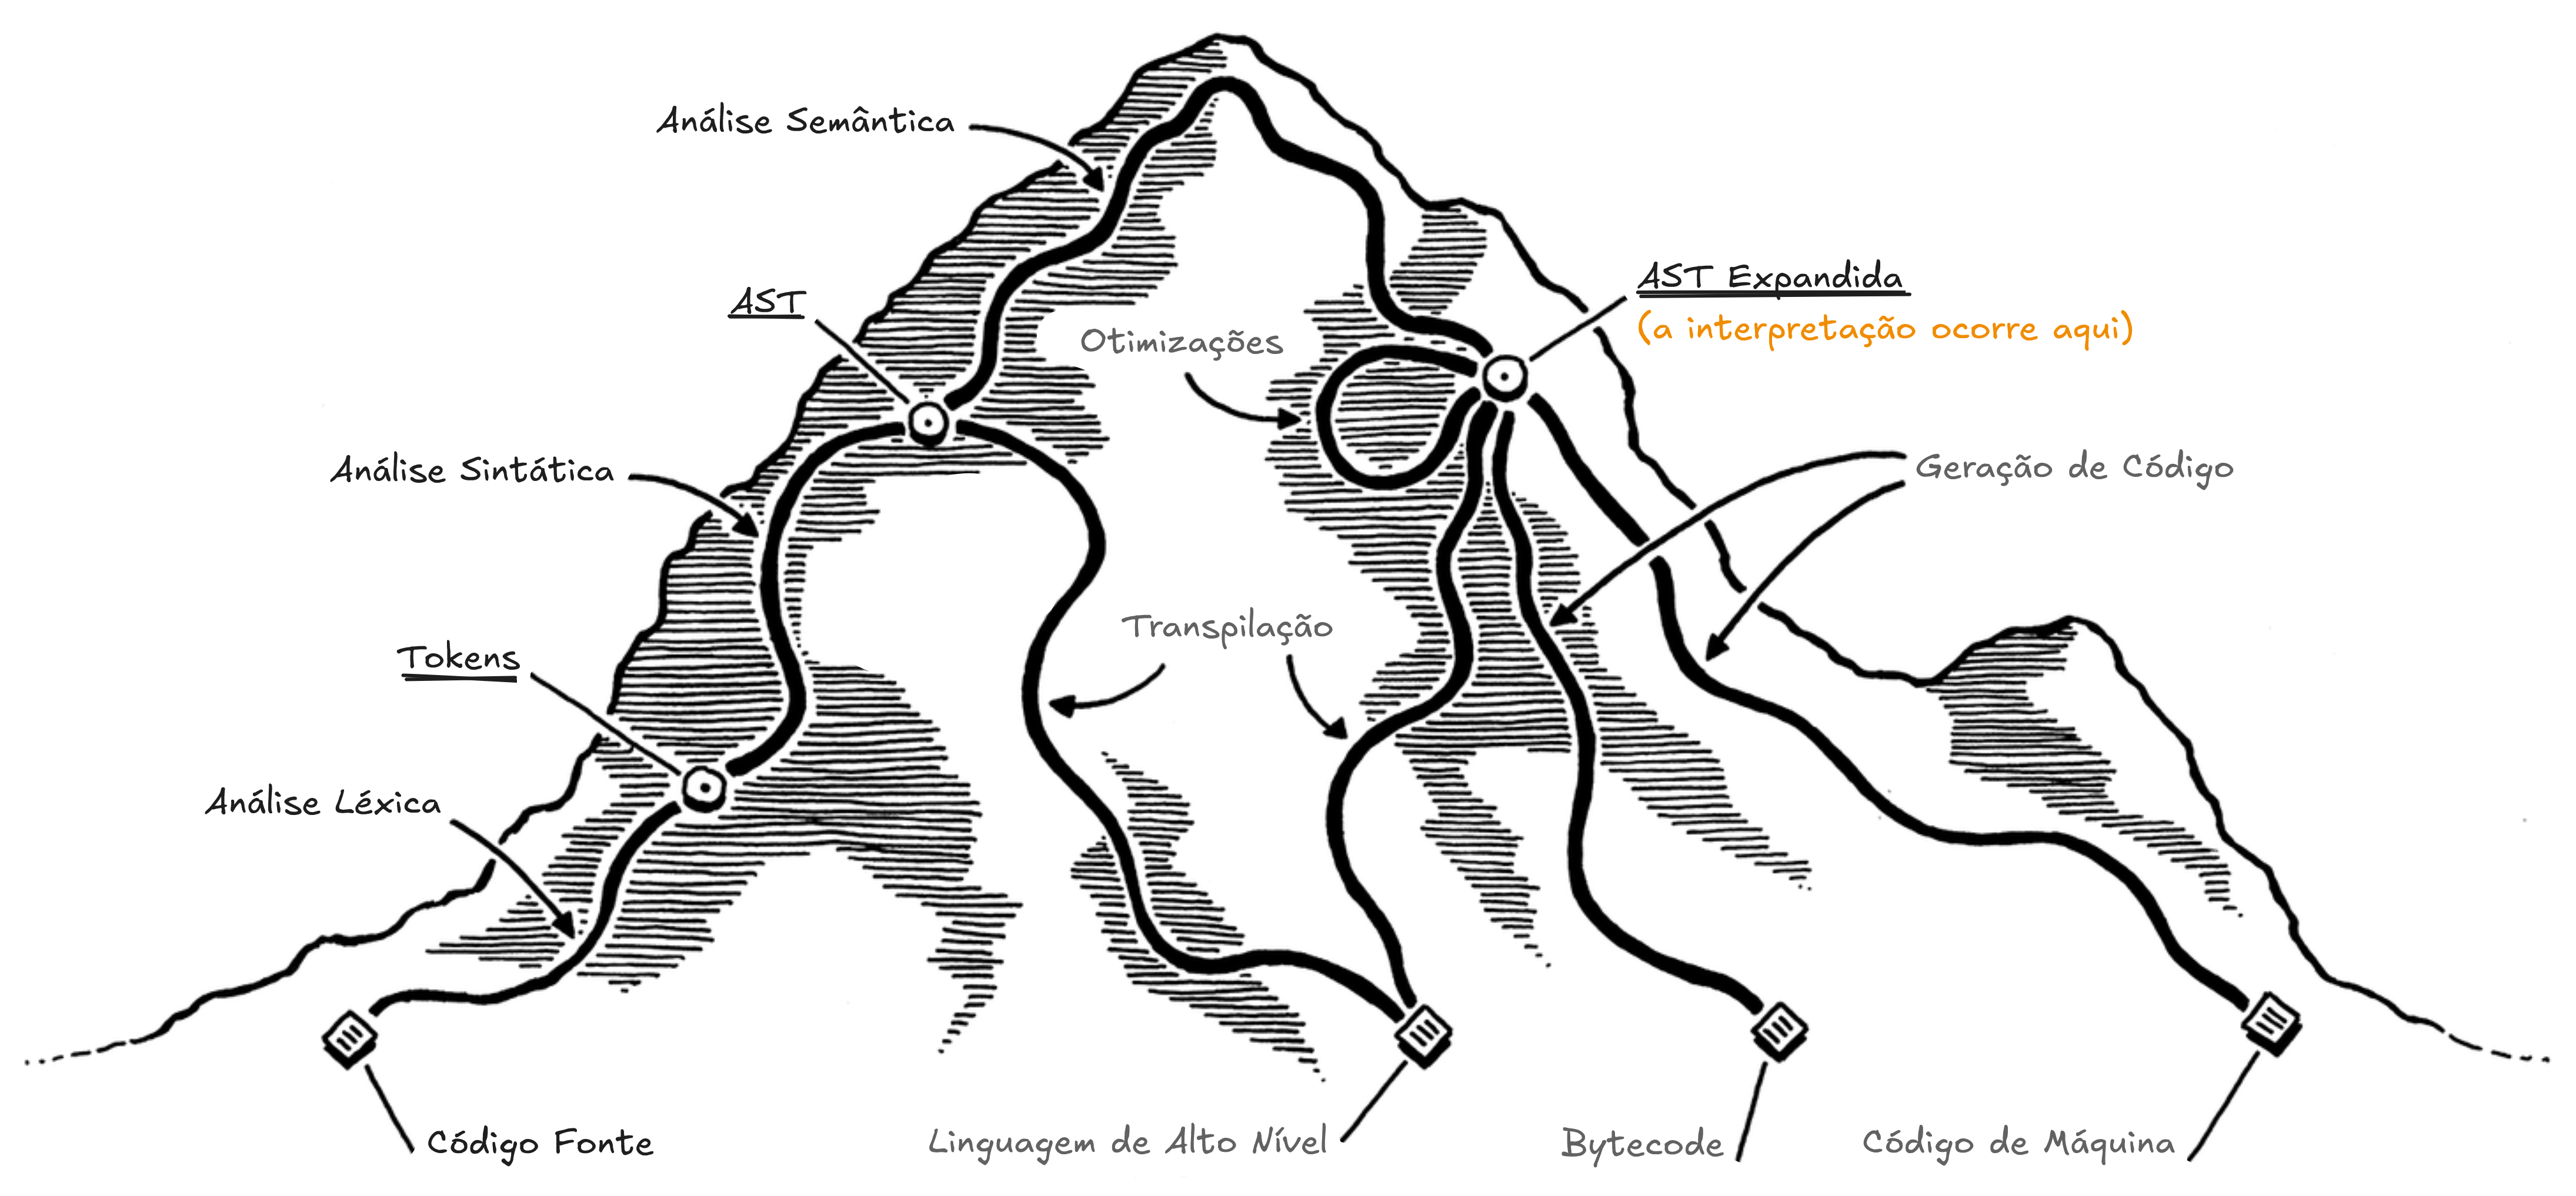
\includegraphics[height=0.275\textheight]{mapa_interpretador}
	\caption{Mapa do território de um interpretador.}
	\fonte{\cite{craftinginterpreters}.}
	\label{fig:mapa_interpretador}
\end{figure}

A seguir, serão definidas em detalhe cada uma das três principais fases de um interpretador:

\begin{enumerate}
	\item Análise léxica: primeira fase do processo de interpretação, onde as palavras do código fonte são transformadas em tokens, estruturas de dados que armazenam informações sobre cada palavra da gramática da linguagem \cite{craftinginterpreters}. A \autoref{fig:analise_lexica} ilustra o processo, onde o código fonte é mapeado para uma lista de \textit{tokens};

	\begin{figure}[H]
		\centering
		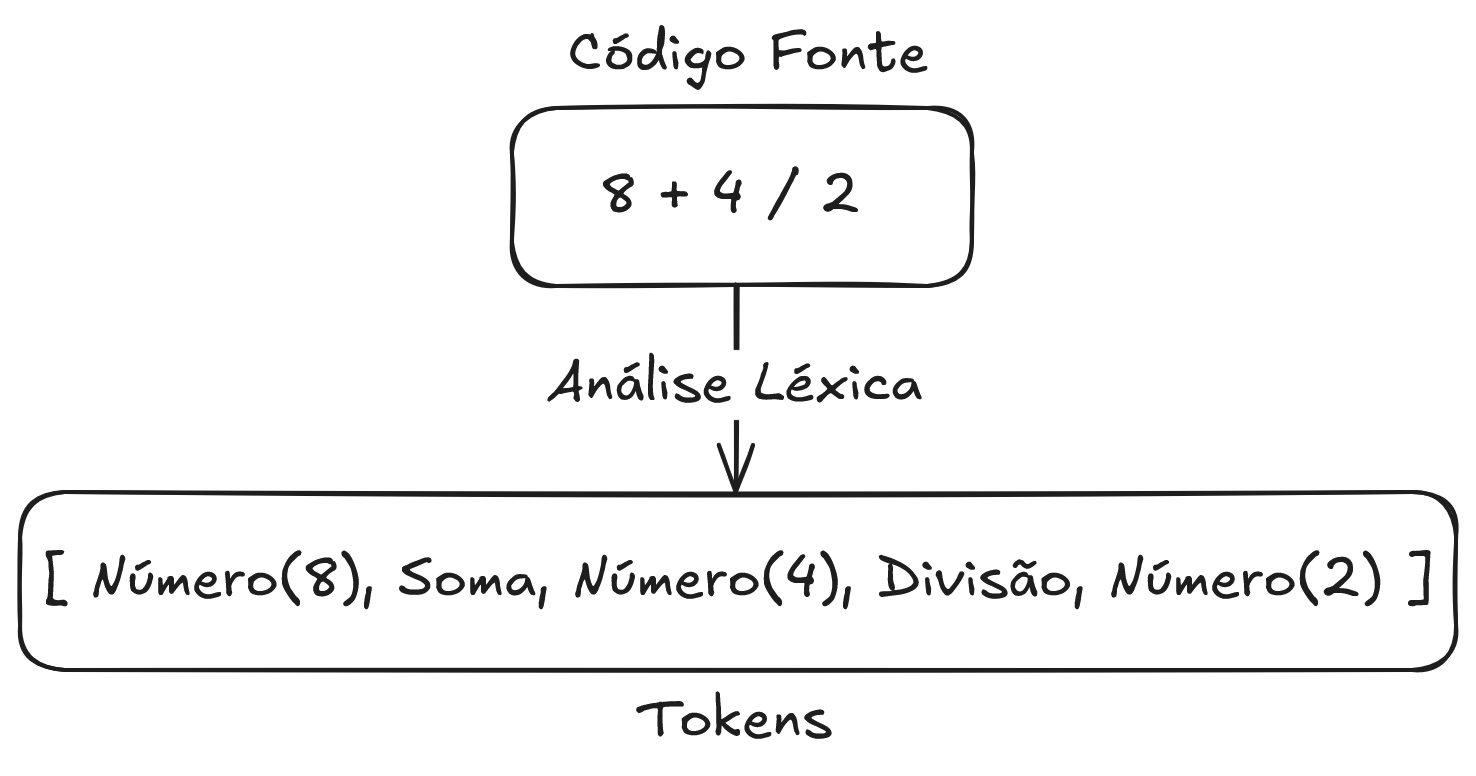
\includegraphics[height=0.2\textheight]{analise_lexica}
		\caption{Código fonte sendo mapeado para uma lista de tokens pela análise léxica.}
		\fonte{Elaboração própria com base em \citeonline{craftinginterpreters}.}
		\label{fig:analise_lexica}
	\end{figure}

	\item Análise sintática: segunda fase do processo de interpretação, onde os tokens gerados na fase anterior são organizados em uma árvore sintática abstrata (do inglês, \textit{abstract syntax tree} — AST), que representa a hierarquia estrutural do código de acordo com as regras gramaticais da linguagem \cite{craftinginterpreters}. A \autoref{fig:analise_sintatica} ilustra o processo, onde os \textit{tokens} são organizados em uma AST, criando uma hierarquia que reflete a estrutura do código fonte;

	\begin{figure}[H]
		\centering
		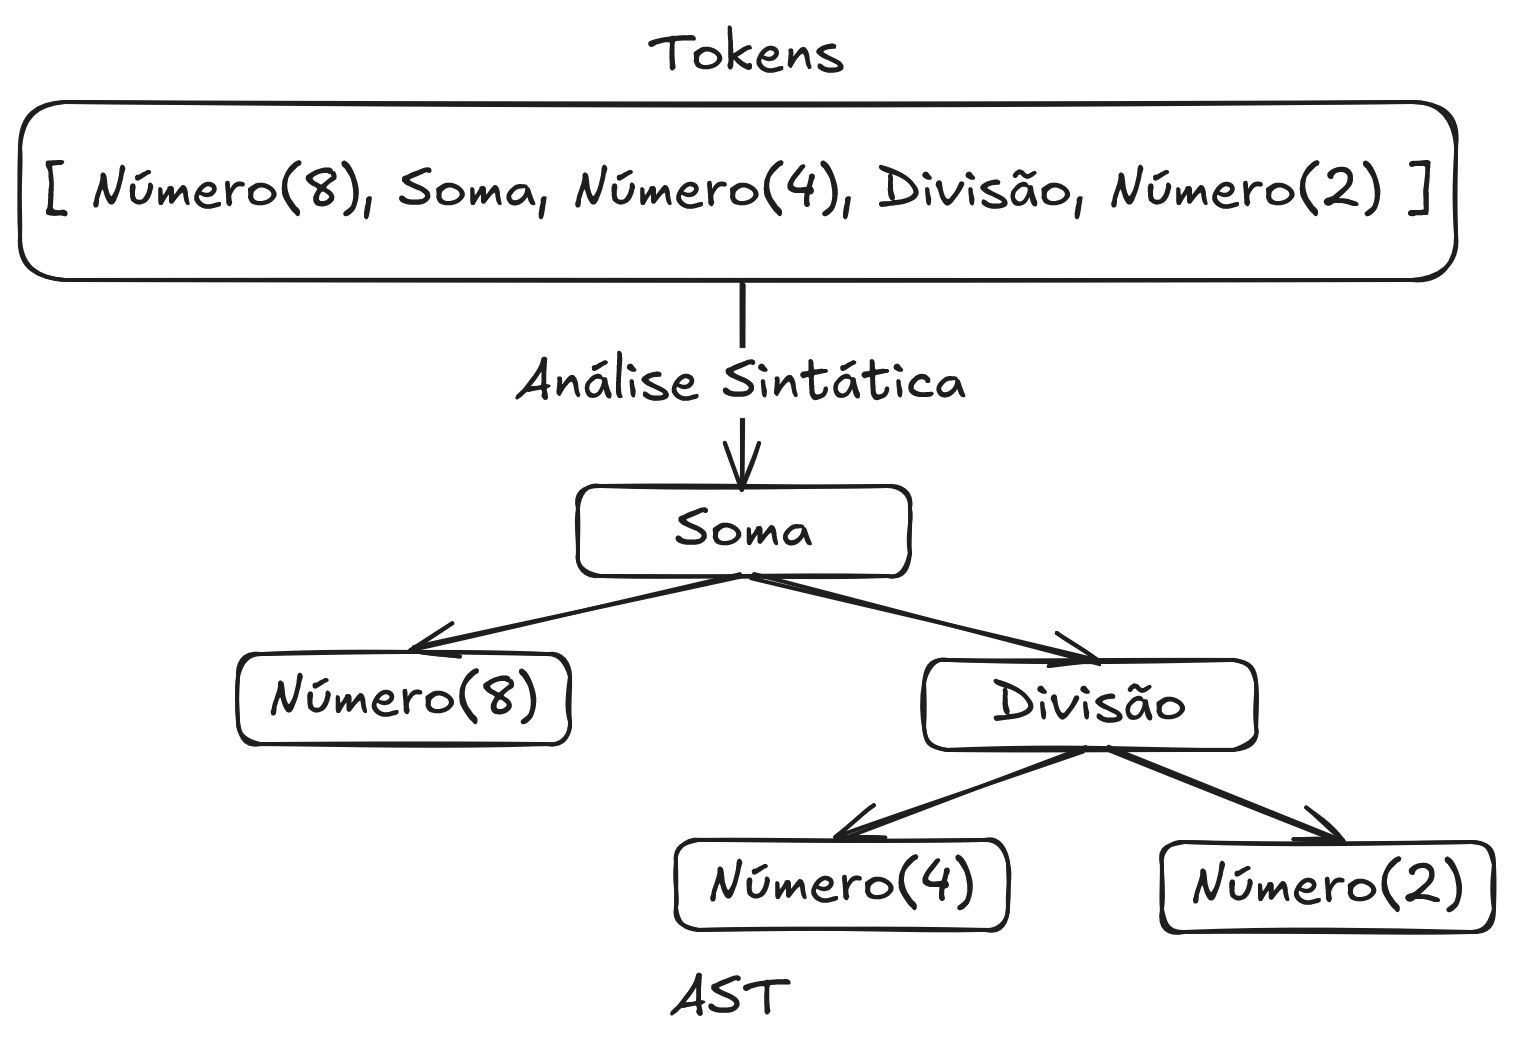
\includegraphics[height=0.27\textheight]{analise_sintatica}
		\caption{Tokens sendo organizados em uma AST pela análise sintática.}
		\fonte{Elaboração própria com base em \citeonline{craftinginterpreters}.}
		\label{fig:analise_sintatica}
	\end{figure}

	\item Interpretação: última fase do processo de interpretação, onde a AST gerada na fase de análise sintática é percorrida e executada. Durante esta fase, o interpretador avalia expressões, atualiza o estado do programa e executa funções \cite{craftinginterpreters}. A \autoref{fig:interpretacao} ilustra o processo, onde a AST é percorrida e executada pelo interpretador, resultando no número 10.

	      \begin{figure}[H]
		      \centering
		      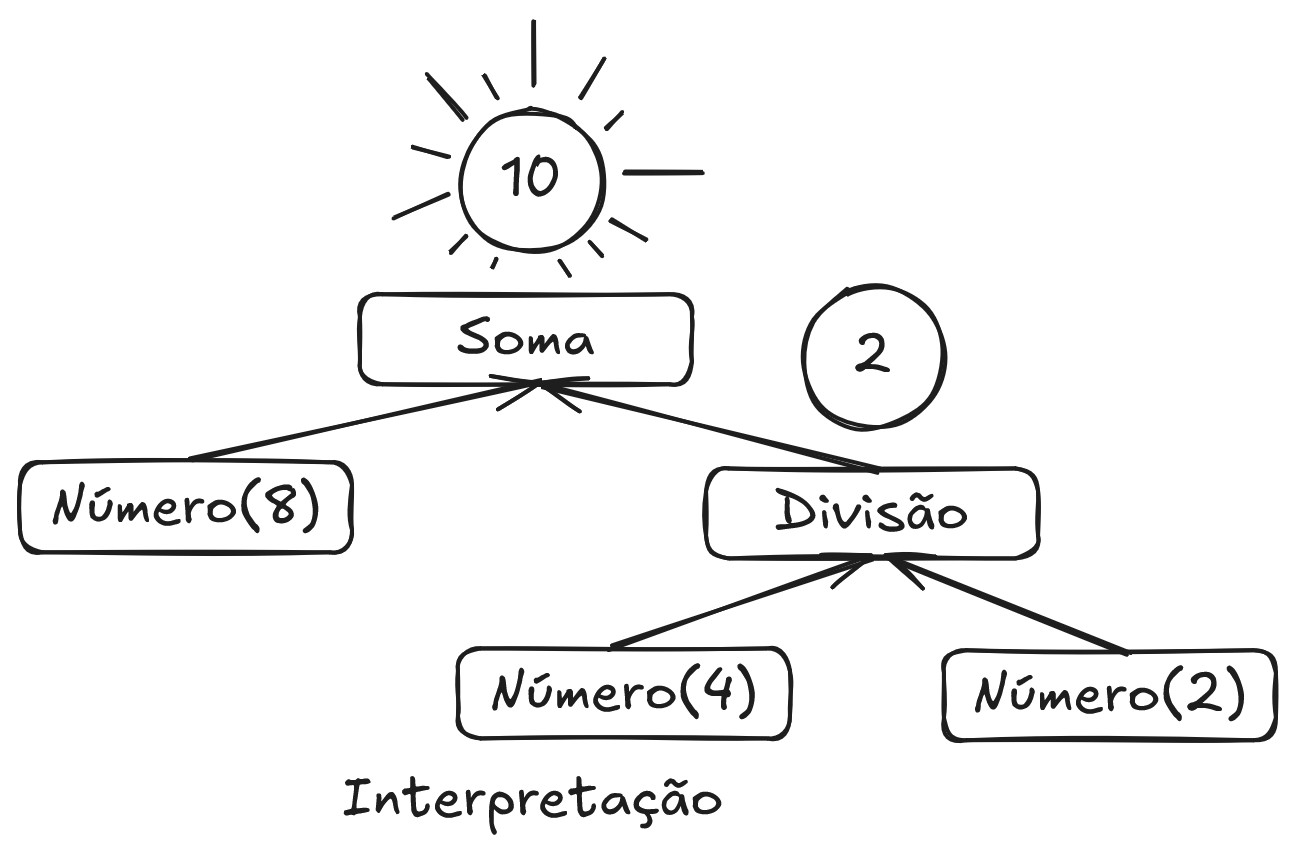
\includegraphics[height=0.25\textheight]{interpretacao}
		      \caption{AST sendo percorrida e executada pela fase de interpretação.}
		      \fonte{Elaboração própria com base em \citeonline{craftinginterpreters}.}
		      \label{fig:interpretacao}
	      \end{figure}
\end{enumerate}
